\documentclass[12pt]{report}
\usepackage[utf8]{inputenc}
\usepackage{a4}
%\usepackage[none]{hyphenat} %hyphenation destroys code linewrapping
\sloppy
\usepackage{parskip} %no indentation after paragraphs
\usepackage{afterpage} %for using \afterpage{\clearpage} (don't push images to the end of a chapter)
\usepackage{makeidx}
\usepackage[numbers]{natbib}
\usepackage{picins} %provides precise control over the placement of inline graphics
\usepackage{setspace}
\usepackage{titlesec}
\usepackage{dsfont} %math symbols
\usepackage{tabularx}
\usepackage{floatflt} %float text around figures and tables
\usepackage{enumitem} %resume counting from previous enumerate block
\usepackage{amsmath,amssymb}
\usepackage[format=default,font=footnotesize,labelfont=bf]{caption}
\usepackage{listings} %for listing source code
\usepackage{color}
\usepackage{float} % for [H] after floats
\usepackage{url}
\usepackage{graphicx} 
\usepackage{todonotes}
\usepackage[automake]{glossaries}
\newglossary[slg]{symbolslist}{syi}{syg}{Symbols}
\makeglossaries
\newacronym{SA}{SA}{Sample Abbreviation}
 % all abbreviations
\newglossaryentry{symb:N}{sort={3},
name={$\mathbb N$},
first={first $\mathbb N$},
text={additional $\mathbb N$},
description={Set of natural numbers},
type=symbolslist} % all symbols
\glsaddall[types=\acronymtype]
\usepackage{listings}
\usepackage{color}
\definecolor{gray}{rgb}{0.4,0.4,0.4}
\definecolor{darkblue}{rgb}{0.0,0.0,0.6}
\definecolor{cyan}{rgb}{0.0,0.6,0.6}
\definecolor{dkgreen}{rgb}{0,0.6,0}
\definecolor{gray}{rgb}{0.5,0.5,0.5}
\definecolor{mauve}{rgb}{0.58,0,0.82}
\definecolor{bat-bg}{rgb}{.16,.19,.2}
\definecolor{bat-norm}{rgb}{.9,.9,.9}
\definecolor{bat-comm}{rgb}{.4,.45,.48}
\definecolor{bat-kw}{rgb}{.57,.78,.39}
\definecolor{bat-str}{rgb}{.2,.38,.62}
\usepackage[autostyle]{csquotes}
\usepackage{subcaption}
\usepackage[ruled,lined,linesnumbered, noend]{algorithm2e}
\usepackage{algorithmicx}
\usepackage{algpseudocode}
\usepackage[]{algorithm2e}
\usepackage{multirow}
\usepackage{rotating}
\usepackage[toc,page]{appendix}
\usepackage{CJKutf8}
\usepackage{longtable}
\usepackage{adjustbox}
\usepackage{url}
\usepackage{pgfplots}
\usepackage{pgfplotstable}

\lstdefinestyle{myScalastyle}{
  frame=tb,
  language=scala,
  aboveskip=3mm,
  belowskip=3mm,
  showstringspaces=false,
  columns=flexible,
  basicstyle={\small\ttfamily},
  numbers=none,
  numberstyle=\tiny\color{gray},
  keywordstyle=\color{blue},
  commentstyle=\color{dkgreen},
  stringstyle=\color{mauve},
  frame=single,
  breaklines=true,
  breakatwhitespace=true,
  tabsize=3,
}

\lstdefinestyle{batch}{
    language={[WinXP]command.com},
    commentstyle=\color{bat-comm},
    keywordstyle=\color{bat-kw},
    keywords=[2]{@},
    keywords=[3]{\%1,\%~2,\%3,\%4, \%params\%, \%url\%, \%redirect\%},
    keywords=[4]{curl},
    keywordstyle=[2]\color{bat-at},
    keywordstyle=[3]\color{bat-str},
    keywordstyle=[4]\color{bat-cmd} 
}

\setlength{\extrarowheight}{10pt}

\lstset{
  basicstyle=\ttfamily,
  columns=fullflexible,
  frame=single,
  breaklines=true,
  postbreak=\mbox{\textcolor{red}{$\hookrightarrow$}\space},
}

\titleformat{\paragraph}[hang]{\normalfont\bfseries}{\theparagraph}{.5em}{}

\makeindex
\frenchspacing
\sloppy
\pagestyle{headings}
\textwidth16cm
\textheight22cm
\topmargin0cm
\oddsidemargin0cm
\evensidemargin0cm

\newcommand\tab[1][1cm]{\hspace*{#1}}

\newcommand{\bildklein}[3]{  
	\begin{figure}[hp]
	\begin{center}
	\includegraphics[width=0.5\textwidth]{#1}
	\end{center}
	\caption[#2]{#3}
	\end{figure}
}	
\newcommand{\bildgross}[3]{  
	\begin{figure}[hp]
	\begin{center}
	\includegraphics[width=0.95\textwidth]{#1}
	\end{center}
	\caption[#2]{#3}
	\end{figure}
}

\input{figures/tumlogo}

\begin{document}

\hoffset=5mm
\thispagestyle{empty}
\begin{center}
	\bigskip \bigskip \bigskip 
	\oTUM{6.0cm} \\
	\vspace*{0.8cm}
	{\huge \bf Technische Universität} \\
	\bigskip
	{\huge \bf München} \\
	\bigskip \bigskip \bigskip
	{\huge \bf Fakultät für Informatik} \\
	\bigskip \bigskip \bigskip
	{\Large \bf Master's Thesis in Information Systems} \\
	\bigskip \bigskip \bigskip \bigskip \bigskip
	{\Large  Bitcoin-like Blockchain Simulation System} \\        
	\bigskip \bigskip \bigskip \bigskip
	{\Large Fabian Schüssler} \\    
	\bigskip
	\begin{figure}[ht]
	\centering \includegraphics[width=0.2\linewidth]{figures/infologo.jpg}
	\end{figure}
	\bigskip 
\end{center}
\vfill

\newpage
\hoffset=5mm
\thispagestyle{empty}
\begin{center}
	\bigskip \bigskip \bigskip 
	\oTUM{6.0cm} \\
	\vspace*{0.8cm}
	{\huge \bf Technische Universität} \\
	\bigskip
	{\huge \bf München} \\
	\bigskip \bigskip \bigskip
	{\huge \bf Fakultät für Informatik} \\
	\bigskip \bigskip \bigskip
	{\Large \bf Master's Thesis in Information Systems} \\
	\bigskip \bigskip \bigskip \bigskip \bigskip
	{\Large Bitcoin-like Blockchain Simulation System} \\
	\bigskip \bigskip \bigskip
	{\Large Bitcoin-ähnliches Blockchain Simulationssystem} \\
	\bigskip
\end{center}
\vfill
\begin{tabular}{ll}
{\Large \bf Author:} & {\Large Fabian Schüssler} \\\\
{\Large \bf Supervisor:} & {\Large Prof. Dr. Hans-Arno Jacobsen} \\\\
{\Large \bf Advisor:} & {\Large Pezhman Nasirifard} \\\\
{\Large \bf Submission:} & {\Large xx.xx.20xx}
\end{tabular}

\newpage	
\thispagestyle{empty}
\hoffset=0mm
\vspace*{\fill}
\noindent I confirm that this master's thesis is my own work and I have documented all sources and material used.\\\\
München, xx.xx.20xx\\\\\\\\\\\\
\noindent \textit{(Fabian Schüssler)}

\newpage
\thispagestyle{empty}
\null

\newpage
\thispagestyle{empty}
\hoffset=0mm
\section*{Abstract}	
\begin{spacing}{1.2}
Despite the recent \$600 billion crash and the high volatility of the whole cryptocurrency market, interest in development and research on blockchains is growing. Reaching the scalability of more traditional payment processors like PayPal or VISA is still a hard problem for decentralized peer-to-peer networks like bitcoin. Heated debates about scalability solutions led to the creation of hardforks like bitcoin cash. For users to better understand the impact of changes to the bitcoin protocol on scalability and security and to find optimal solutions, we propose Bitcoin-like Blockchain Simulation System (BBSS). BBSS is a configurable bitcoin-like blockchain simulator. Its focus is on the visualisation of the simulation results to make every blockchain detail easy to understand. With block size limits, transaction fees, Segregated Witness and other features the Scalability Problem can be analysed. The optional attacks double-spending and transaction spam allow examination of security properties. The design and architecture allow large-scale simulations in a comparatively short amount of time.
\end{spacing}
 
\newpage
\thispagestyle{empty}
\hoffset=0mm
\section*{Inhaltsangabe}
\begin{spacing}{1.2}
Trotz des kürzlichen 600 Milliarden US-Dollar Kursabsturz und der hohen Volatilität des gesamten Kryptowährungsmarkt wächst das Interesse in Entwicklung und Forschung von Blockketten. Die Skalierbarkeit von eher traditionellen Zahlungsabwicklern wie PayPal oder VISA zu erreichen ist immer noch ein schwieriges Problem für dezentralisierte Rechner-zu-Rechner Netzwerke wie Bitcoin. Lebhafte Debatten über Verbesserungen der Skalierbarkeit haben zu Hardforks wie Bitcoin Cash geführt. Damit Benutzer die Auswirkungen von Veränderungen am Bitcoin Protokoll besser verstehen können und um optimale Lösungen zu finden, schlagen wir das Bitcoin-ähnliche Blockchain Simulationssystem vor (BBSS). BBSS ist ein konfigurierbarer Bitcoin-ähnlicher Blockchain Simulator. Der Fokus liegt auf die Visualisierung der Simulationsergebnisse, um jedes Detail der Blockchain einfach verständlich zu machen. Mit Beschränkungen der Blockgröße, Transaktionsgebühren, SegWit und anderen Erweiterungen kann das Problem der Skalierbarkeit analysiert werden. Die optionalen Angriffe wie doppelte Ausgabe und Transaktionsmüll erlaubt die Untersuchung von Sicherheitseigenschaften. Das Design und die Architektur erlauben Simulationen mit vielen Netzwerkteilnehmern in einer im Vergleich mit anderen Lösungen kurzen Zeit.
\end{spacing}

\newpage
\thispagestyle{empty}
\hoffset=0mm
\section*{Acknowledgment}	
\begin{spacing}{1.2}
\input{sections/acknowledgment}
\end{spacing}

\newpage
\setcounter{page}{1}
\hoffset=0mm
\fboxsep 0mm

\tableofcontents
\setcounter{tocdepth}{2}

\listoffigures
\addcontentsline{toc}{chapter}{List of Figures}

\listoftables
\addcontentsline{toc}{chapter}{List of Tables}

\printglossary[type=\acronymtype,style=long ,title=Abbreviations, toctitle=Abbreviations,nonumberlist]
\printglossary[type=symbolslist,style=long ,title=Symbols, nonumberlist]
\addcontentsline{toc}{chapter}{Abbreviations}

\newpage
\setlength{\baselineskip}{3ex}
\begin{spacing}{1.15}
\chapter{Introduction} 
\label{chapter:introduction}
There are papers describing blockchain technology as a disruptive innovation \cite{atzori2015blockchain}. The \textit{Harvard Business Review} argues blockchain technology is not a disruptive, but a foundational technology \cite{harvardbusinessreview}. Whether blockchain is a disruptive technology or not, it is largely agreed upon that blockchain technology has immense potential and can revolutionize business and redefine companies and economies. But there are still lots of barriers. Currently and in the last years, blockchain technologies such as Bitcoin \cite{nakamoto2012bitcoin}, Ethereum \cite{buterin2014ethereum}, IOTA \cite{Newcomb:2017:ICI:3133850.3133860} or Hyperledger fabric \cite{Androulaki:2018:HFD:3190508.3190538} are a very hot topic. According to the Gartner Hype Cycle Blockchain technology was undergoing the peak of inflated expectation in 2017 \cite{gartner}. Price and market capitalization changes of cryptocurrencies are widely covered by the media. This shows Blockchain technologies are believed to have a great potential and a big variety of new use cases. 

Blockchain technology enables decentralized consensus and can be used for record keeping. Bitcoin is the first digital currency to solve the double-spending problem without the need of a trusted authority. One of the main problems of Bitcoin or in general of blockchains is the low maximum amount of possible processed transactions per second. Additionally, the Bitcoin community disagrees about how to solve this scalability problem. It already split into multiple communities with different approaches and Bitcoin forks.

VIBES (Visualizations of Interactive, Blockchain, Extended Simulations) is a blockchain simulator, which allows fast, scalable and configurable network simulations on a single computer without any additional resources. It was developed in a master thesis by Lyubomir Stoykov \cite{vibes} and is the foundation of this master thesis.

\section{Motivation} 
\label{sec:motivation}
The implications of blockchain protocol changes on key figures like scalability or security are difficult to predict. The reasons are complex relationships between the different parameter of the blockchain network, which can change the way nodes interact with each other or how blocks are handled. This may lead to getting the impression, the blockchain network is a black box. A configurable simulator can help to answer questions about scalability or security.

The goal of this master thesis is to improve VIBES to make more realistic bitcoin-like blockchain simulations possible. In the future, BBSS could be used by developers or heavy blockchain users to simulate changes to different blockchains, so it can help the bitcoin community to agree on bitcoin improvement proposals (BIP).

\section{Problem Statement} 
\label{sec:problemStatement}
Ideally, the users of VIBES could specify their Bitcoin-like Blockchain Simulation. VIBES then presents the results of the simulation in a very detailed and still easily understandable way.

In reality, VIBES does not yet support Bitcoin-like Blockchain Simulations. The Generic Simulations lack defining traits of Bitcoin like maximum block size, SegWit, transaction incentives or attack scenarios. Also, other important metrics are not yet displayed.

To achieve our goals VIBES needs to be changed in a way to allow multiple strategies in the front- and backend, while still having good maintainability of the code. A Bitcoin-like Blockchain Simulation needs to be implemented next to the existing Generic Simulation.

These extensions can improve the quality of the simulations and the use cases of VIBES. For example, the implications of Segwit2x could be analysed. Maybe these extensions could also make it possible to realistically simulate the current bitcoin blockchain with an as similar as possible configuration.

The focus of this master thesis is to implement a Bitcoin-like Blockchain Simulation with all important features to make the simulations as realistic as possible, to make it possible to simulate attacks like double-spending and to visualise all important outputs.

The approach is evaluated by six key figures: correctness, speed,
scalability, flexibility, extensibility and powerful visuals.

\section{Approach}
 \label{sec:approach}
The presented goals should be achieved while maintaining and extending the design and architecture of the existing VIBES framework, which are described in Chapter \ref{chapter:relatedWork}. The Bitcoin-like Blockchain Simulation fast-forwards the whole network ahead of time and skips heavy computations such as solving a block. The actor model is used to achieve simulation at the event level. The Coordinator or also called MasterActor takes the role of an application-level scheduler to make fast-forwarding possible. The Coordinator and other actors need to be adjusted for the Bitcoin-like Blockchain Simulation and attack scenarios. For the visual side, the pattern of Atomic Design \cite{atomicdesign} is maintained to add new visualisations to a high-quality and composable user interface.

\section{Contribution}
 \label{sec:contribution}
Before BBSS, there was no multi-purpose bitcoin simulator with good visualisations. BBSS makes bitcoin-like blockchains easy to understand and allows the optimization of bitcoin-like blockchains in scalability and security. Different scalability related changes like block size limit, SegWit or transaction incentives can be analysed. BBSS also allows the simulation of attacks like double-spending and transaction spam. The changes were implemented in a way to enable good maintainability to adjust the simulation to future changes of the bitcoin protocol or to add new attacks.

\section{Organization}
 \label{sec:organization}
The structure of the thesis begins with this chapter as an introduction. The second chapter describes the background and the theoretical foundations which are necessary for the understanding of this thesis. The Chapter \ref{chapter:relatedWork}: Related Work presents related research papers and the architecture and design of VIBES on which this thesis builds on. And it also shows other related works and puts this work into perspective. Chapter \ref{chapter:approach} describes the approach and implementation details are explained. Developers or users of the simulator can use Chapter \ref{chapter:approach} as documentation to explain questions about the behaviour of the simulations. Chapter \ref{chapter:evaluation}: Evaluation uses empirical and theoretical analysis to test the implementation according to our predefined criteria. In the last chapter, the status, conclusions and, suggestions for future work are summarised.


\chapter{Background} 
\label{chapter:background}

Background concepts required for understanding the thesis. 
\chapter{Related Work}
\label{chapter:relatedWork}

Related work materials 

\chapter{Approach}\label{chapter:approach}
Approach

\section{Lazy Logging}

\subsection{Prerequisites}

\subsection{Design and Architecture}

\subsection{Implementation}

\section{Block size limit}
The introduction of a block size limit allows a more accurate simulation of the Bitcoin network.

\subsection{Prerequisites}

\subsection{Design and Architecture}

\subsection{Implementation}

\section{Alternative history attack}

\subsection{Prerequisites}

To simulate an alternative history attack additional \textbf{configuration parameters} are necessary. These parameters are used for the actual simulation of the attack, the calcuation of the success probability of the attack and the maximum safe transaction value.

\begin{itemize}
\item \textit{isAlternativeHistoryAttack}: if an alternative history attack is simulated as a boolean
\item \textit{hashrate}: attacker's hashrate as a percentage of the total hashrate of the Bitcoin Network
\item \textit{confirmations}: the amount of confirmations the attacked merchants are waiting for to accept a transaction
\item \textit{attackDuration}: the attacker gives up after mining a certain amount of blocks and not suceeding or if it is not possible anymore to surpass the level of the public blockchain
\item \textit{discountOnStolenGoods}: discount of the stolen goods by the attacker, a value from 0 (= full discount) to 1 (= no discount)
\item \textit{amountOfAttackedMerchants}: the attack is carried out against a certain amount of merchants at the same time
\item \textit{blockReward}: current block reward in BTC
\end{itemize}

\subsection{Design and Architecture}

\subsubsection{Simulating the attack}

In the following the attacker's nodes, blockchain or blocks are interchangeably described as \textit{evil} and the public networks' nodes as \textit{good}.\linebreak

The solution for the simulation of an alternative history attack selects nodes as attacking nodes according to the attacker's hashrate as a percentage of the total Bitcoin Network.
The good and the evil nodes both can mine the genesis block. The genesis block is then the first block in both the good and the evil blockchain. For simplicity we assume that the attacker successfully sent the transactions to the attacked merchants in the second block of the public blockchain. Immediately after the genesis block is mined, the evil nodes start mining together on their own evil blockchain. It is necessary for all nodes to update their neighbour nodes to only have their corresponding nodes as neighbours. For example in the case of a low amount of evil nodes and a low amount of neighbours... Since the attacker of course doesn't want his...\linebreak

Finally the success of the simulated attack is decided if the attacker's blockchain level can surpass the public's blockchain level after waiting for the Merchants confirmation and before the attack duration ends.

\subsubsection{Calculating the success probability  \cite{doublespending}}

Before the formula to calculate the success probability of an alternative history attack is shown, the variables need to be defined.\linebreak
...

\begin{equation}
p + q = 1
\end{equation}

\includegraphics[scale=0.7]{successProbability.PNG} 

The formula for $q < p$ is transformed to the following formula to be used in the implementation.

\begin{equation}
r = 1-\sum\limits_{m=0}^n \frac{(m+n-1)!}{m!\,(n-1)!}(p^nq^m-p^mq^n)
\end{equation}

\subsubsection{Calculating the safe transaction value  \cite{doublespending}}

\begin{equation}
k \alpha v - (1 - r)(kv + oB) = kv( \alpha + r - 1) - (1 - r)oB
\end{equation}

\subsection{Implementation}



VConf ...

\begin{minipage}{\linewidth}
\begin{lstlisting}[style=myScalastyle]
object VBlock extends LazyLogging {
  def createWinnerBlock(node: VNode, timestamp: DateTime): VBlock = {
    var maxTransactionsPerBlock : Int = 0
    var processedTransactionsInBlock: Set[VTransaction] = Set.empty

    if (VConf.strategy == "BITCOIN_LIKE_BLOCKCHAIN") {
      // todo think about if to implement SegWit (maxBlockWeight vs maxBlockSize)
      maxTransactionsPerBlock = Math.floor(VConf.maxBlockSize / VConf.transactionSize).toInt

      // sorts the transaction pool by the transaction fee
      processedTransactionsInBlock = node.transactionPool.toSeq.sortWith(_.transactionFee > _.transactionFee).take(maxTransactionsPerBlock).toSet

      // sets confirmation status of transaction true
      processedTransactionsInBlock.foreach { _.confirmation = true }

      // sets confirmation level of transaction
      processedTransactionsInBlock.foreach { _.confirmationLevel = node.blockchain.size }
    } else {
      maxTransactionsPerBlock = node.transactionPool.size
      processedTransactionsInBlock = node.transactionPool
    }

    VBlock(
      id = UUID.randomUUID().toString,
      origin = node,
      transactions = processedTransactionsInBlock,
      level = node.blockchain.size,
      timestamp = timestamp,
      recipients = ListBuffer.empty,
      transactionPoolSize = node.transactionPool.size
    )
  }
}
\end{lstlisting}
\end{minipage}
\chapter{Evaluation}
\label{chapter:evaluation}

For the evaluation of the approach the same six criteria from VIBES are taken: correctness, speed, scalability, flexibility, extensibility and powerful visuals. These criteria must be at least maintained or improved. Additionally, new use cases are showcased.

\section{Correctness}
The evaluation of the correctness of the simulator's frontend output is essential. By validating the output of the frontend we also validate the output of the backend.

Some parts of the evaluations are sample testing for consistency between the input parameters, expected and simulated or calculated output. Other parts are empirically tested.

For the calculation of the probability of a successful double spend and the maximal safe transaction value sample testing is used. For validating the success probability of simulated double spends empirical testing is applied.

\subsection{Block Size Limit}

\subsubsection{Average block size =< Non-SegWit maximal block size}

\subsubsection{Total number of processed transactions =< Non-SegWit maximal transactions per block * Blocks}

\subsection{Segregated Witness}

\subsubsection{Average block size =< SegWit maximal block weight =< SegWit theoretical block weight limit}

\subsubsection{Total number of processed transactions =< SegWit maximal transactions per block * Blocks}

\subsection{Simulated and Expected Transaction Incentives}
If the number of process transactions per block is smaller than the maximum number of transactions per block, then the transaction incentives have no impact. For the evaluation of transaction incentives we take a look at the Figures \ref{fig:TransactionIncentives1}, \ref{fig:TransactionIncentives2} and \ref{fig:TransactionSpam} which are all based on scenarios with full blocks.

\subsubsection{Transactions with higher fees should have a better confirmation status}
The first expectation is transaction with higher transaction fees should have preference over transaction with lower transaction fees, therefore in the transaction confirmation status chart the lower transaction fees should have a higher percentage of unconfirmed transactions. The simulated results confirm this expectation.

\subsubsection{Transactions with higher fees should have a shorter average transaction confirmation time}
The second expectation is transactions with higher transaction fees should have a shorter average transaction confirmation time. The simulated results confirm this expectation.

\subsection{Transaction Spam}
The Screenshot Transaction Spam \ref{fig:TransactionSpam} shows the simulated results which match the following expected results.

\subsubsection{No transaction confirmed with transaction fee below the target}
No transaction below the target transaction fee is expected. The charts about the transaction confirmation status and the average transaction confirmation time and the flood attack summary show that no confirmed transaction has a transaction fee below the target.

\subsubsection{All blocks are full}
One of the requirements of a transaction spam attack is that the blocks need to be full to block the transactions with fees below the target. All blocks in Figure \ref{fig:TransactionSpam} are full, except for the genesis block. There are 28 blocks, the maximum number of transactions per block is 100, so 2.700 transactions are expected and simulated.

\subsubsection{Flood attack transaction buffer is not shrinking}
To guarantee that no transaction below the target is confirmed, the flood attack transaction buffer should not decrease and stay constant. The number of pending flood attack transactions stays constant in the pending transaction chart.

\subsection{Expected and Simulated Transactions per Second}

For the evaluation of correctness of the transactions per second (tps) of our simulation, the formula for the calculation of \textit{tps} is compared to the implementation.

\begin{equation}
\text{tps} = \text{transactions per block} / \text{block time}
\end{equation}

Since the \textit{tps} for the whole simulation is an important key metric, the division is not done for one block, but instead for all blocks.

\begin{minipage}{\linewidth}
\begin{lstlisting}[style=myScalastyle]
    var tps: Double = longestChainNumberTransactions.toDouble / secondsBetween(VConf.simulationStart, VConf.simulateUntil).getSeconds.toDouble
\end{lstlisting}
\end{minipage}

As can be seen, the formulas are identical and therefore the result should be correct. Sample testing is done to check for implementation errors.

\subsubsection{Sample with a Simulation Duration of Six Hours}

For the first sample a short simulation of six hours is chosen. The chosen block time is 567 seconds and the chosen throughput is 105 transactions per block (\textit{tpb}).

Calculation of the expected total processed transactions \textit{pt}:
\begin{equation}
\textit{pt} = 6 \text{h} / 567 \text{sec} * 105 \text{tpb} = 6*60*60/567 * 105 = 4000
\end{equation}

Calculation of the expected \textit{tps}:
\begin{equation}
\text{tps} = 4000 \text{transactions} / 6 \text{h} = 0.185
\end{equation}

\begin{figure}[!htb]
\centering
\includegraphics[height=0.3\textwidth]{"figures/Testing/tps 1".PNG}
\caption{Screenshot Transactions per Second - 6h Simulation Duration\label{fig:tpsSimulation6h}}
\end{figure}

\begin{table}[ht]
    \caption{Simulated and expected results of transactions per second: Sample with 6h simulation duration\label{table:tps6hsimulation}}
\centering
\begin{adjustbox}{width=0.8\textwidth}
    \begin{tabular}{| l | r | r |}
    \hline
    \textbf{Metric} & \textbf{Simulation} & \textbf{Expectation}\\ \hline
    Block time & 692 & 567\\ \hline
    Total number of processed transactions & 3000 & 4000 \\ \hline
    Transactions per second & 0.14 & 0.185\\ \hline
    \end{tabular}
\end{adjustbox}
\end{table} 

As can be seen in Table \ref{table:tps6hsimulation}, for such a short simulation the tps is off by about 30\%. One reason for this significant difference is the difference in the block time between the simulated and expected values. This can be due to variance. To reduce block time variance a longer simulation time is chosen as a second sample.

The parameters for reproduction can be found in Chapter \ref{6hoursURL}.

\subsubsection{Sample with a Duration of 48 Hours}

For the second sample a longer simulation of 48 hours is chosen. The chosen block time is still 567 seconds and the chosen throughput is also still 105 transactions per block (\textit{tpb}).

Calculation of the expected total processed transactions:
\begin{equation}
\text{pt} = 48h / 567 \text{sec} * 105 \text{tpb} = 48*60*60/567 * 105 = 32000
\end{equation}

Of course the expected tps stays the same, since only the simulation duration parameter has been changed.

\begin{figure}[!htb]
\centering
\includegraphics[height=0.3\textwidth]{"figures/Testing/tps 2".PNG}
\caption{Screenshot Transactions per Second - 48h Simulation Duration\label{fig:tpsSimulation48h}}
\end{figure}

\begin{table}[ht]
    \caption{Simulated and expected results of transactions per second: Sample with 48h simulation duration\label{table:tps48hsimulation}}
\centering
\begin{adjustbox}{width=0.8\textwidth}
    \begin{tabular}{| l | r | r |}
    \hline
    \textbf{Metric} & \textbf{Simulation} & \textbf{Expectation}\\ \hline
    Block time & 539 & 567\\ \hline
    Total number of processed transactions & 
31700 & 32000 \\ \hline
    Transactions per second & 0.18 & 0.185\\ \hline
    \end{tabular}
\end{adjustbox}
\end{table} 

It can be observed in the second comparative table \ref{table:tps48hsimulation}, that a longer simulation duration leads the simulated block time to be closer to the expected block time. As a result the simulated \textit{tps} is close to the expected value.

The parameters for reproduction can be found in Chapter \ref{48hoursURL}.

\subsection{Expected and Calculated Probability of a Successful Double-Spending Attack}
\label{subsection:evalCalcDoubleSpending}
The probability of a successful double-spending attack is tested with five samples and the results are compared to the Figure \ref{fig:doubleSpend} from the research paper \textit{Analysis of Hashrate-Based Double Spending} \cite{doublespending}.

The variable q stands for the hashrate, the variable n is the number of confirmations. The edge cases q = 2\% and n = 1, q = 2\% and n = 10, q = 50\% and n = 1 and q = 50\% and n = 10 are tested as well as the common case of q = 30\% and n = 6.

\begin{table}[ht]
    \caption{Expected and Calculated Probabilities of a Successful Double-Spending Attack\label{table:doubleSpendingSimulatedAndCalculatedSuccessProbability}}
\centering
\begin{adjustbox}{width=0.8\textwidth}
    \begin{tabular}{| l | r | r | r | r |}
    \hline
    \textbf{Sample} & \textbf{n} & \textbf{q} & \textbf{Calculated Probability} & \textbf{Expected Probability} \\ \hline
    a & 2 & 1 & 4\% & 4\% \\ \hline
    b & 2 & 10 & 0\% & 0\% \\ \hline
    c & 50 & 1 & 100\% & 100\% \\ \hline
    d & 50 & 10 & 100\% & 100\% \\ \hline
    e & 30 & 6 & 15.645\% & 15.645\% \\ \hline
    \end{tabular}
\end{adjustbox}
\end{table}

All mentioned test cases in Figure \ref{fig:testCases} match the expected result.

\begin{figure}[p]
\centering

\subcaptionbox{Sample with input: q = 2\% and n = 1}{\includegraphics[width=0.365\textwidth]{"figures/Testing/q 2 n 1".PNG}}%
\hfill % <-- Separation
\subcaptionbox{Sample with input: q = 2\% and n = 10}{\includegraphics[width=0.365\textwidth]{"figures/Testing/q 2 n 10".PNG}}%
\hfill % <-- Separation

\vskip\baselineskip

\subcaptionbox{Sample with input: q = 50\% and n = 1}{\includegraphics[width=0.365\textwidth]{"figures/Testing/q 50 n 1".PNG}}%
\hfill % <-- Separation
\subcaptionbox{Sample with input: q = 50\% and n = 10}{\includegraphics[width=0.365\textwidth]{"figures/Testing/q 50 n 10".PNG}}%
\hfill % <-- Separation

\vskip\baselineskip

\subcaptionbox{Sample with input: q = 30\% and n = 6}{\includegraphics[width=0.365\textwidth]{"figures/Testing/q 30 n 6".PNG}}%
\hfill % <-- Separation

\caption{Screenshots Success Probability of Double-Spending\label{fig:testCases}}
\end{figure}

\subsection{Expected and Calculated Maximal Safe Transaction Value}
For the test of the maximal safe transaction value the samples from the evaluation of the successful double spend probability are reused and compared to Figure \ref{fig:maximalSafeTransactionValue}.

The additional input parameters were:

\begin{itemize}
\item Attack duration: 20 Blocks
\item Discount on stolen goods: 1
\item Attacked merchants: 5
\item Block reward: 12.5 BTC
\end{itemize}

Compared to the \textit{Analysis of Hashrate-Based Double Spending} paper the block reward was updated from 25 BTC to the current block reward of 12.5 BTC. This means the maximal safe transaction values need to be doubled to compare them with the correct values.

\begin{table}[ht]
    \caption{Expected and Calculated Maximal Safe Transaction Values (MSTV)\label{table:doubleSpendingSimulatedAndCalculatedMSTV}}
\centering
\begin{adjustbox}{width=0.65\textwidth}
    \begin{tabular}{| l | r | r | r | r |}
    \hline
    \textbf{Sample} & \textbf{n} & \textbf{q} & \textbf{Calculated MSTV} & \textbf{Expected MSTV} \\ \hline
    a & 2 & 1 & 1199 BTC & 1200 BTC \\ \hline
    b & 2 & 10 & $\infty$ BTC & $\infty$ BTC \\ \hline
    c & 50 & 1 & 0 BTC & 0 BTC \\ \hline
    d & 50 & 10 & 0 BTC & 0 BTC \\ \hline
    e & 30 & 6 & 269 BTC & 269.5 BTC \\ \hline
    \end{tabular}
\end{adjustbox}
\end{table}

Ignoring minor rounding differences in samples (a) and (e), all test cases in Figure \ref{fig:testCases} match the expected result. The sample with $\infty$ BTC is a special case, the frontend displays $\infty$ BTC in the case of receiving 2,147,483,647 BTC which is the maximal possible 32-bit signed integer value. 2,147,483,647 BTC is much more than the hard supply limit of 21 million BTC.

\subsection{Expected and Simulated Success Probability of Double Spending}
\label{subsection:evalDoubleSpending}
The success probability for the scenario with q = 30\% and n = 6 is reused from Chapter \ref{subsection:evalCalcDoubleSpending}.

For the empirical testing of double-spending a script was used, it can be found in Chapter \ref{evalDoubleSpending} for reproduction. It starts the simulation, waits for a certain time to let the simulation finish and repeats this for a total of 100 times.

\begin{table}[ht]
\caption{Double-spending outcomes and their simulated and expected probabilities\label{table:doubleSpendingSimulatedAndExpected}}
\centering
\begin{adjustbox}{width=1\textwidth}
    \begin{tabular}{| l | r | r | r |}
    \hline
    \textbf{Outcome} & \textbf{Occurrences} & \textbf{Simulated probability} & \textbf{Expected probability} \\ \hline
    Attack neither successful nor failed & 45 & - & - \\ \hline
    Attack successful & 8 & 15.09\% & 15.645\% \\ \hline
    Attack failed & 47 & 84.91\% & 84.355\% \\ \hline
    \textbf{TOTAL} & \textbf{100} & \textbf{100\%} & \textbf{100\%} \\ \hline
    \end{tabular}
\end{adjustbox}
\end{table}

After counting the occurrences of the outcomes in the logfile, they were summarized in Table \ref{table:doubleSpendingSimulatedAndExpected}. All simulations were finished in the specified time. The undecided attacks are ignored for the calculation of the probabilities. It is assumed that the unfinished simulations have a similar probability distribution like the finished ones. The simulated probability of the double-spending attack is with 15.09\% very close to the expected probability of 15.645\%, which was calculated in Chapter \ref{subsection:evalCalcDoubleSpending}. Hereby is shown that the simulation of double-spending has the correct success probability.

\section{Speed}
To make sure there are no significant performance losses introduced by the implementation of bitcoin, we compare the simulation results from BBSS with VIBES.

\section{Scalability}
The block size limit, the block weight limit and the target transaction fee in the case of a flood attack are in $O(1)$ and do not effect the performance, except for requiring increasing memory if the throughput is higher than the maximal transactions per block.

For examining the effect of the hashrate in case of a double-spending attack on the scalability, multiple simulations were executed. Figure \ref{figure:limitations} show there is no significant difference in simulation duration because of a varying hashrate.

\begin{figure}
\centering
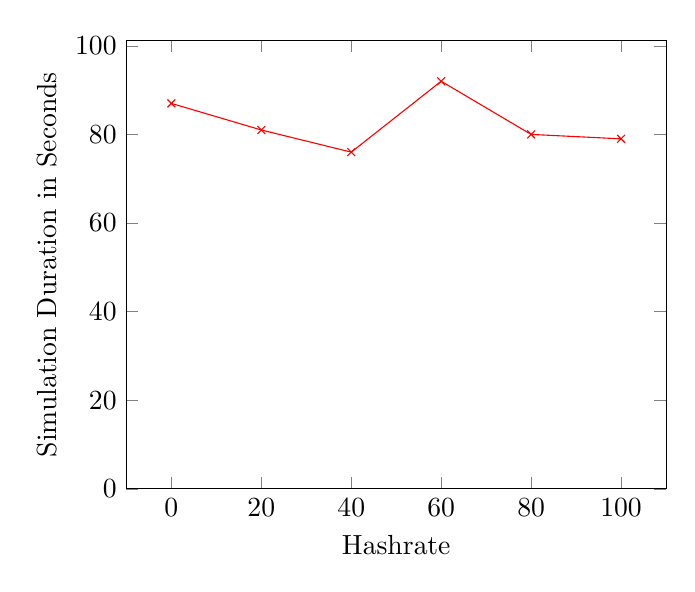
\begin{tikzpicture}
	\begin{axis}[
	    ymin=0,
		xlabel=Hashrate,
		ylabel=Simulation Duration in Seconds]
	\addplot[color=red,mark=x] coordinates {
		( 0,87)
		( 20,81)
		( 40,76)
		( 60,92)
		( 80,80)
		(100,79)
	};
	\end{axis}
\end{tikzpicture}
\caption{Effect of Hashrate on Simulation Duration\label{figure:limitations}}
\end{figure}

\section{Limitations of Speed and Scalability}
There are certain limitations on the simulator. One of the goals of the simulator is that the execution time of the simulation is shorter than the simulated duration. With increasing nodes and transactions, there is a point when the execution time equals the simulation time. In this chapter we want to examine this relationship and the resulting speedup ratio. The speedup ratio is the simulated duration divided by the execution duration.

All computations were done on a Home PC with Windows Ultimate 64-bit, Intel i7-4770 CPU @ 3.40 GHz and 16.0 GB 1600 MHz DD3.

The simulations were done with an equal number of nodes and transactions. This seems to be a good ratio for the simulator, which allows lots of parallel computation. 

The Table \ref{table:limitations} and the Figure \ref{figure:limitations2} shows the results of the simulations and the declining speedup ratio with increasing nodes and transactions. The values in the table should be considered as approximations, since only one simulation per number of nodes and transactions was done and the block time deviations can have an impact on the speedup ratio. One of the consequences deriving from this table is that it is not feasible to do a simulation with the configuration of the real-world bitcoin network with ten thousand nodes and one thousand tpb on a Home PC.

\begin{figure}
\centering
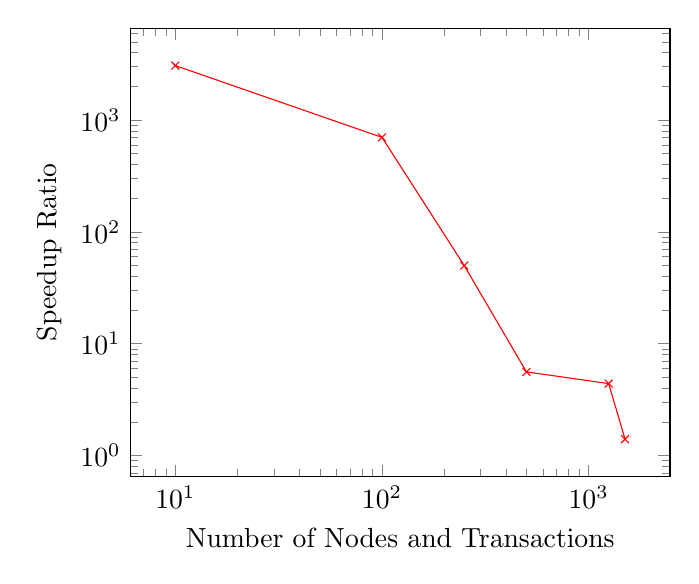
\begin{tikzpicture}
	\begin{loglogaxis}[
		xlabel=Number of Nodes and Transactions,
		ylabel=Speedup Ratio]
	\addplot[color=red,mark=x] coordinates {
		(  10,3070  )
		( 100, 700  )
		( 250,  50  )
		( 500,   5.6)
		(1250,   4.4)
		(1500,   1.4)
	};
	\end{loglogaxis}
\end{tikzpicture}
\caption{Effect of Hashrate on Simulation Duration\label{figure:limitations2}}
\end{figure}

\begin{table}[ht]
\caption{Effect of Number of Nodes and Transactions on the Speedup Ratio \label{table:limitations}}
\centering
\begin{adjustbox}{width=1\textwidth}
    \begin{tabular}{| r | r | r | r |}
    \hline
    \textbf{Number of Nodes and Transactions} & \textbf{Simulation Duration in Seconds} & \textbf{Execution Duration in Seconds} & \textbf{Speedup Ratio} \\ \hline
    10 & 21480 & 7 & 3070 \\ \hline
    100 & 21120 & 30 & 700 \\ \hline
    250 & 19140 & 373 & 50 \\ \hline
    500 & 6900 & 1228 & 5.6 \\ \hline
    1250 & 3045 & 697 & 4.4 \\ \hline
    1500 & 3060 & 2188 & 1.4 \\\hline
    \end{tabular}
\end{adjustbox}
\end{table}

Of course, other configuration parameters than nodes and transactions like block size limit or block weight limit have a limiting impact due to the increasing memory requirement.

\subsection{Realistic Bitcoin Network Simulation with AWS}

Amazon Web Service (AWS) is used to find out if it is actually possible to simulate a bitcoin network with ten thousand nodes and thousand tpb. The instance typ t2.2xlarge has a similar performance to the used Home PC and therefore doesn't have the required performance. The instance type p3.2xlarge was chosen, since it is advertised as "high performance computing" and as "ideal platform for technical simulations".

\begin{figure}[h]
\centering
\includegraphics[width=1\textwidth]{"figures/p32xlarge".PNG}
\caption{Screenshot AWS p3.2xlarge
\label{fig:aws}}
\end{figure}

Using various tools we asumme the following configuration parameters:
\begin{itemize}
\item strategy=BITCOIN\_LIKE\_BLOCKCHAIN
\item simulateUntil={1 hour}
\item blockTime=600
\item numberOfNeighbours=15
\item numberOfNodes=10000 \cite{configuration_node}
\item neighboursDiscoveryInterval=3000
\item latency=900
\item transactionSize=700 \cite{configuration_transaction_size}
\item maxBlockSize=0
\item throughput=1300 \cite{configuration_tpb}
\item transactionWeight=1400
\item maxBlockWeight=4000000
\item networkBandwidth=1
\item transactionPropagationDelay=150
\item hashRate=0
\item confirmations=0
\item transactionFee=0
\end{itemize}

With these configuration parameters the simulator uses only about 20\% CPU. This means realistic parameters do not allow lots of parallel computing. The number of neighbours seems to be too small, since the stale block rate is very high which leads slower than real-time simulation.

The numbers of neighbours needs to be between 19 and 22 to reach all nodes after four or five levels of block propagation. In VIBES the optimal number of neighbours for 100 nodes is 4 to 5 neighbours, which is a similar level of block propagation.

But with 21 neighbours the simulation is slower than real-time, the performance of p3.2xlarge is not sufficient. As shown in the Evaluation Chapter of VIBES, increasing the neighbours increases the execution time linearly. All these parameters like nodes, throughput and neighbours scale linearly, but put together they increase the execution effort too heavily.

\section{Flexibility}
asdf

\section{Extensibility}
asdf

\section{Powerful Visuals}

\begin{figure}[p]
\centering
\includegraphics[width=1\textwidth]{"figures/configuration".PNG}
\caption{Screenshot Configuration
\label{fig:configuration}}
\end{figure}

\begin{figure}[p]
\centering
\includegraphics[width=1\textwidth]{"figures/simulation-0-0".PNG}
\caption{Screenshot Simulation - Part 1
\label{fig:simulation1}}
\end{figure}

\begin{figure}[p]
\centering
\includegraphics[width=1\textwidth]{"figures/simulation-0-1".PNG}
\caption{Screenshot Simulation - Part 2
\label{fig:simulation2}}
\end{figure}

\section{Use Cases}
This thesis made new use cases possible, some of which are presented in the following chapter.

\subsection{Optimising Transactions per Second}
Scalability is one of the biggest issues of bitcoin-like blockchains. The simulator could be used to optimised the tps of bitcoin.

\cite{blocksizeincrease}

for example block size increase like in research paper..

\subsection{Securing a Blockchain Merchant}


\subsection{Choosing Transaction Fees}


\subsection{Flood Attack}

\chapter{Summary} \label{chapter:summary}

Summary

\section{Status} 
\label{sec:status}

Final Status of the Thesis

\section{Conclusions}
\label{sec:conclusions}

Concluding remarks of Thesis

\section{Future Work} 
\label{sec:futureWork}

Future Work
\end{spacing}

\newpage
\begin{appendices}
\addtocontents{toc}{\protect\setcounter{tocdepth}{0}}
\chapter{Appendix}

\section{First}

First Appendix

\end{appendices}

\newpage

\def\UrlBreaks{\do\/\do-}

\bibliographystyle{ieeetr}
\bibliography{IEEEabrv,literature}
\end{document}